\documentclass[10pt]{beamer}

  % Math Packages
  \usepackage{amsmath}
  \usepackage{amsthm}
  \usepackage{mathtools}

  % Graphics Packages
  \usepackage{graphicx}
  \usepackage{pgf}
  \usepackage[export]{adjustbox}

  % Colors
  \definecolor{umared}{RGB}{255,74,74}
  \definecolor{mygray}{RGB}{66,66,66}

  % Theme Settings
  \usetheme{metropolis}

  \setbeamercolor{normal text}{fg=mygray}
  \setbeamercolor{alerted text}{fg=umared}
  \setbeamercolor{title text}{fg=mygray}
  \setbeamercolor{title separator}{fg=umared}
  \setbeamercolor{progress bar}{fg=umared}
  \setbeamercolor{frametitle}{bg=umared}

\title{Oracle Taxation Theory}
\logo{
  \makebox[0.13\paperwidth]{\includegraphics[width=1.5cm,keepaspectratio]{Uma_Logo.png} \hfill}
}
\date[]{\today}

\begin{document}

% Title Slide
\begin{frame}
  \titlepage
\end{frame}


% --------------------------------------- %
% Oracle Problem
% --------------------------------------- %
\section{Oracle Problem}

  \begin{frame} \frametitle{Goal}

    UMA's protocols allow synthetic assets to be traded on the blockchain

    \vspace{0.20cm}

    However, to evaluate synthetic assets we must be able to determine asset prices

    \vspace{0.20cm}

    Where can we get these asset prices?

  \end{frame}

  \begin{frame} \frametitle{DVM Structure}

    We propose to use our Data Verification Machine (DVM) to produce these prices

    \vspace{0.20cm}

    \textbf{DVM Summary}:
    \begin{itemize}
      \item Distribute ``vote tokens''
      \item Holders of ``vote tokens'' determine asset prices using a form of Schelling point game
      \item Buy back some amount of ``vote tokens'' from those who own them
      \item These buyback are funded by charging a fee to those who depend on the asset prices
    \end{itemize}

  \end{frame}

  \begin{frame} \frametitle{DVM Risks}

    What are the risks of such a system?

    \vspace{0.20cm}

    \begin{itemize}
      \item \textit{Bribe attack}: Offer rewards to voters if they vote for an incorrect price which
            is dictated to them
      \item \textit{Direct attack}: A single person purchases enough tokens to corrupt the system in
            order to swing asset prices in their favor
      \item \textit{Indirect attack}: Change the reference price that most voters may base their
            votes on (i.e, Bloomberg...)
    \end{itemize}

    Our focus today will be on \textbf{direct attacks}

  \end{frame}


% --------------------------------------- %
% PfC < CoC
% --------------------------------------- %
\section{$\text{PfC} < \text{CoC}$}

  \begin{frame} \frametitle{Preventing Corruption}

    Our corruption prevention strategy revolves around a single inequality

    $$\text{Profit from corruption} < \text{Cost of corruption}$$

    System will be constructed to ensure that it is never economically profitable to perform a
    direct attack

  \end{frame}

  \begin{frame} \frametitle{Notation}

    \begin{itemize}
      \item $p_t$: The price of the vote token in dollars at time $t$
      \item $S_t$: The number of outstanding vote tokens at time $t$
      \item $M_t$: The total margin that depends on the DVM at time $t$
      \item $X_t$: The dollar value of the buybacks administered at time $t$
      \item $r$: The risk-free interest rate
      \item $\gamma$: Fraction of margin that can be stolen when corrupted
      \item $\chi$: The fraction of vote tokens required to corrupt system
    \end{itemize}

  \end{frame}

  \begin{frame} \frametitle{Corruptible price}

    Can show that the price that prevents corruption is

    $$p_t \geq 2 \gamma \frac{M_t}{S_t}$$

  \end{frame}

  \begin{frame} \frametitle{Mechanism for preventing corruption}

    We will prevent corruption by taking actions that influence the price of the ``vote token''

    \vspace{0.25cm}

    Note that, if markets are efficient, then

    $$p_t S_t = E \left[ \sum_{s=0}^{\infty} \left(\frac{1}{1+r} \right)^s X_{t+s} \right]$$

    which means increasing current/future buybacks, while holding the number of tokens constant,
    will increase the current asset price

  \end{frame}


% --------------------------------------- %
% Models
% --------------------------------------- %
\section{Deterministic Steady State Model}

  \begin{frame} \frametitle{Steady state}

    In the steady state model, we consider an environment in which margin is constant,

    $$M_t = \bar{M} \quad \forall t$$

    We would like to know what the minimum amount of fees that can be charged in this environment

  \end{frame}

  \begin{frame} \frametitle{Must collect at least $r \bar{M}$}

    One can show that the minimum buyback that ensures the system is incorruptible is given by

    $$\bar{X} = 2 \gamma \bar{M} r$$

    So, in the baseline case ($\gamma = \frac{1}{2}$),  $\bar{X} = r \bar{M}$

  \end{frame}

  \begin{frame} \frametitle{Result}

    Consider a world in which the following three things are true:

    \begin{enumerate}
      \item Blockchains are widely used and accepted technology
      \item UMA is widely used within DeFi
      \item People believe UMA will be widely used within DeFi
    \end{enumerate}

    Then we believe we can support annualized fees of 2\%-5\%.

  \end{frame}


\section{Deterministic Growth Model}

  \begin{frame} \frametitle{Growth}

    Consider an environment in which the entire history of margin is known and that it is described
    by

    $$M_{t+1} = (1 + g) M_t \left( 1 + \frac{M_t}{\bar{M}} \right) ;\quad M_0$$

  \end{frame}

  \begin{frame} \frametitle{Growth Process}

    \begin{figure}
      \scalebox{0.45}{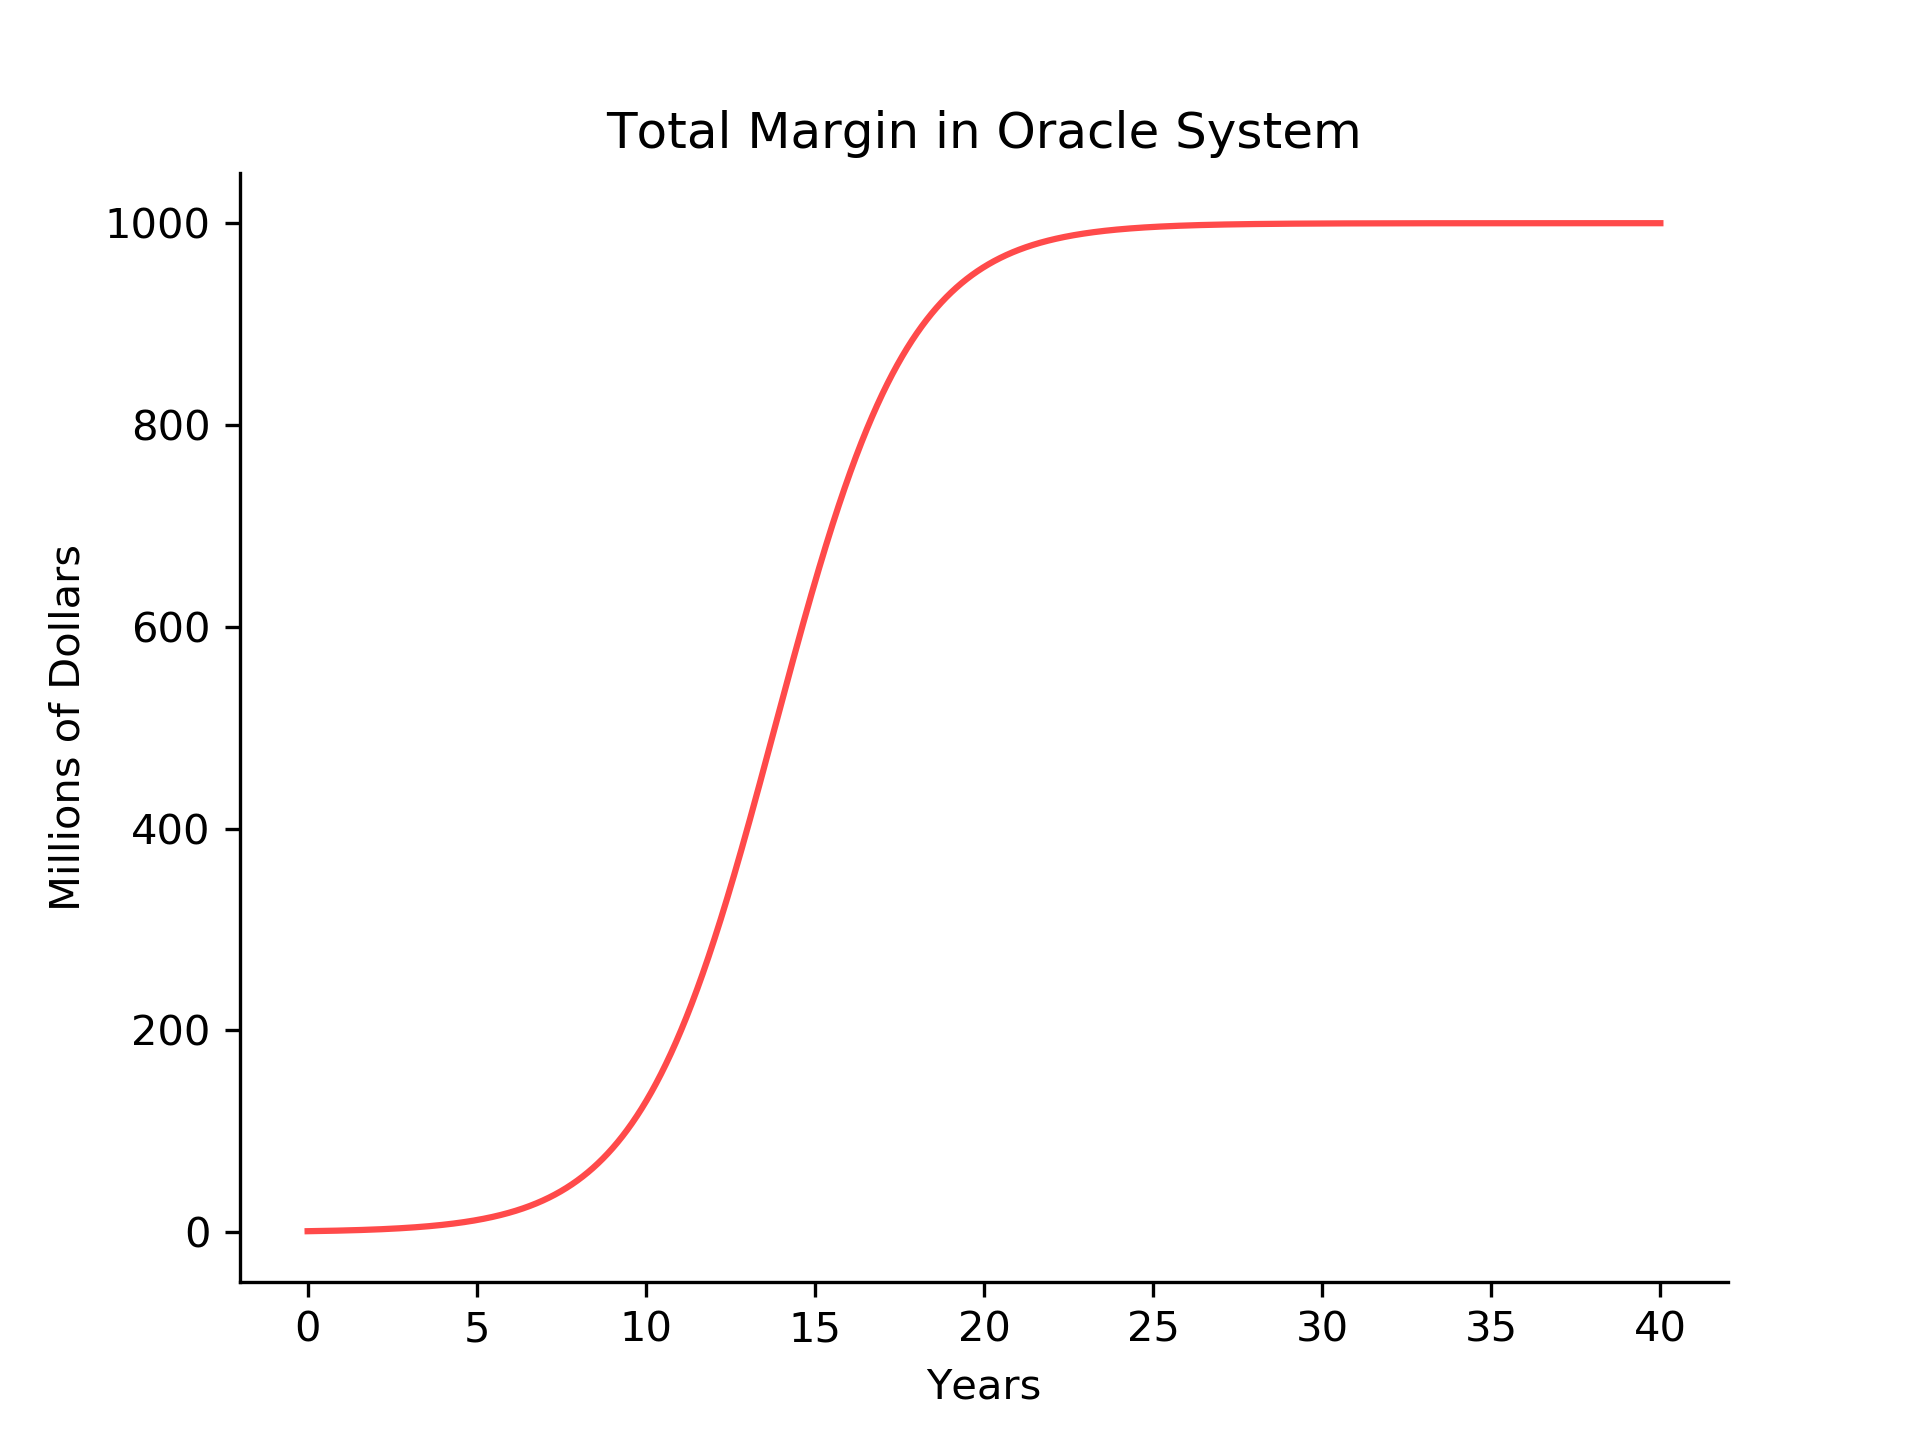
\includegraphics{../notes/TaxationPlanImages/MarginGrowth.png}}
      \label{fig:dg_tax_growth}
    \end{figure}

  \end{frame}

  \begin{frame} \frametitle{Minimize fees subject to no corruption}

    We solve for a buyback policy that allows for minimum amount of fees

    \begin{align*}
      \min_{T_t} \; &E \left[ \sum_{t=0} \left(\frac{1}{1 + r} \right)^t T_t \right] \\
      &\text{subject to} \\
      PfC_t &\leq \frac{1}{2} P_t S_t = \frac{1}{2} E \left[ \sum_{s=0} \left(\frac{1}{1 + r}\right)^s  X_{t + s} \right] \\
      X_{t} &= T_t \\
      0 &\leq T_t \\
      T_t &\leq \bar{\tau} \bar{M} \\
      M_{t+1} &= M_{t} + g M_{t} \left(1 + \frac{M_t}{\bar{M}} \right)
    \end{align*}

  \end{frame}

  \begin{frame} \frametitle{Minimize fees}

    \begin{figure}
      \scalebox{0.45}{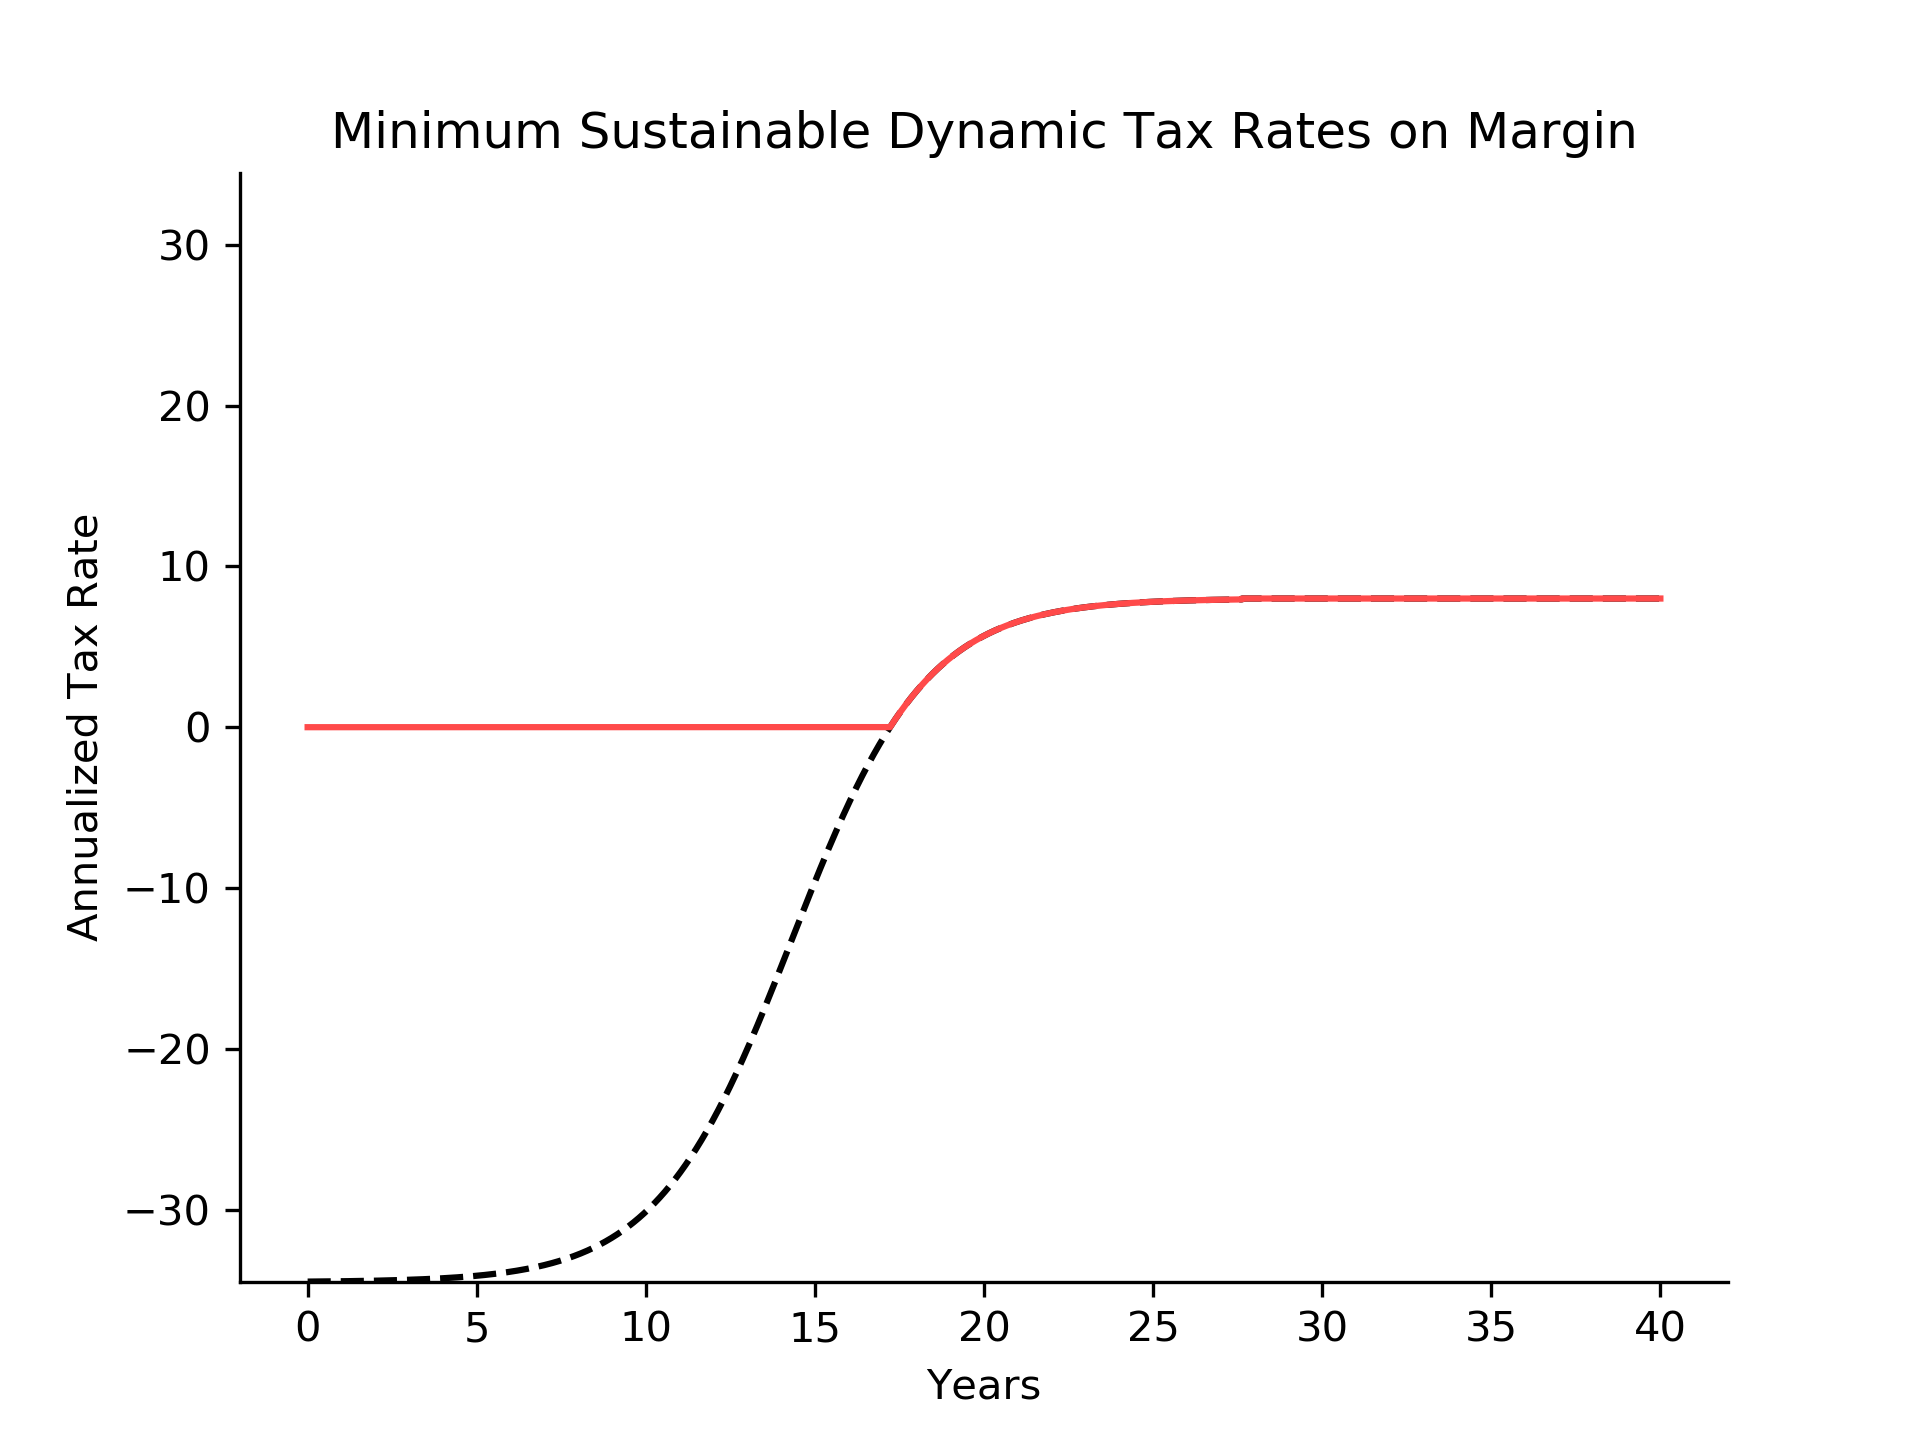
\includegraphics{../notes/TaxationPlanImages/TaxRates.png}}
      \label{fig:dg_tax_growth}
    \end{figure}

  \end{frame}

  \begin{frame} \frametitle{Forward looking fees}

    Our key take-away from the previous graph is that future promises of buybacks are enough to
    support no buybacks for a significant amount of time

    This fact becomes obvious if you stare at the following equation:

    $$\text{CoC}_t = \chi p_t S_t = \chi E \left[ \sum_{s=0}^\infty \left(\frac{1}{1+r}\right) X_{t+s} \right]$$

  \end{frame}

  \begin{frame} \frametitle{Forward looking fees}

    \begin{figure}
      \scalebox{0.3}{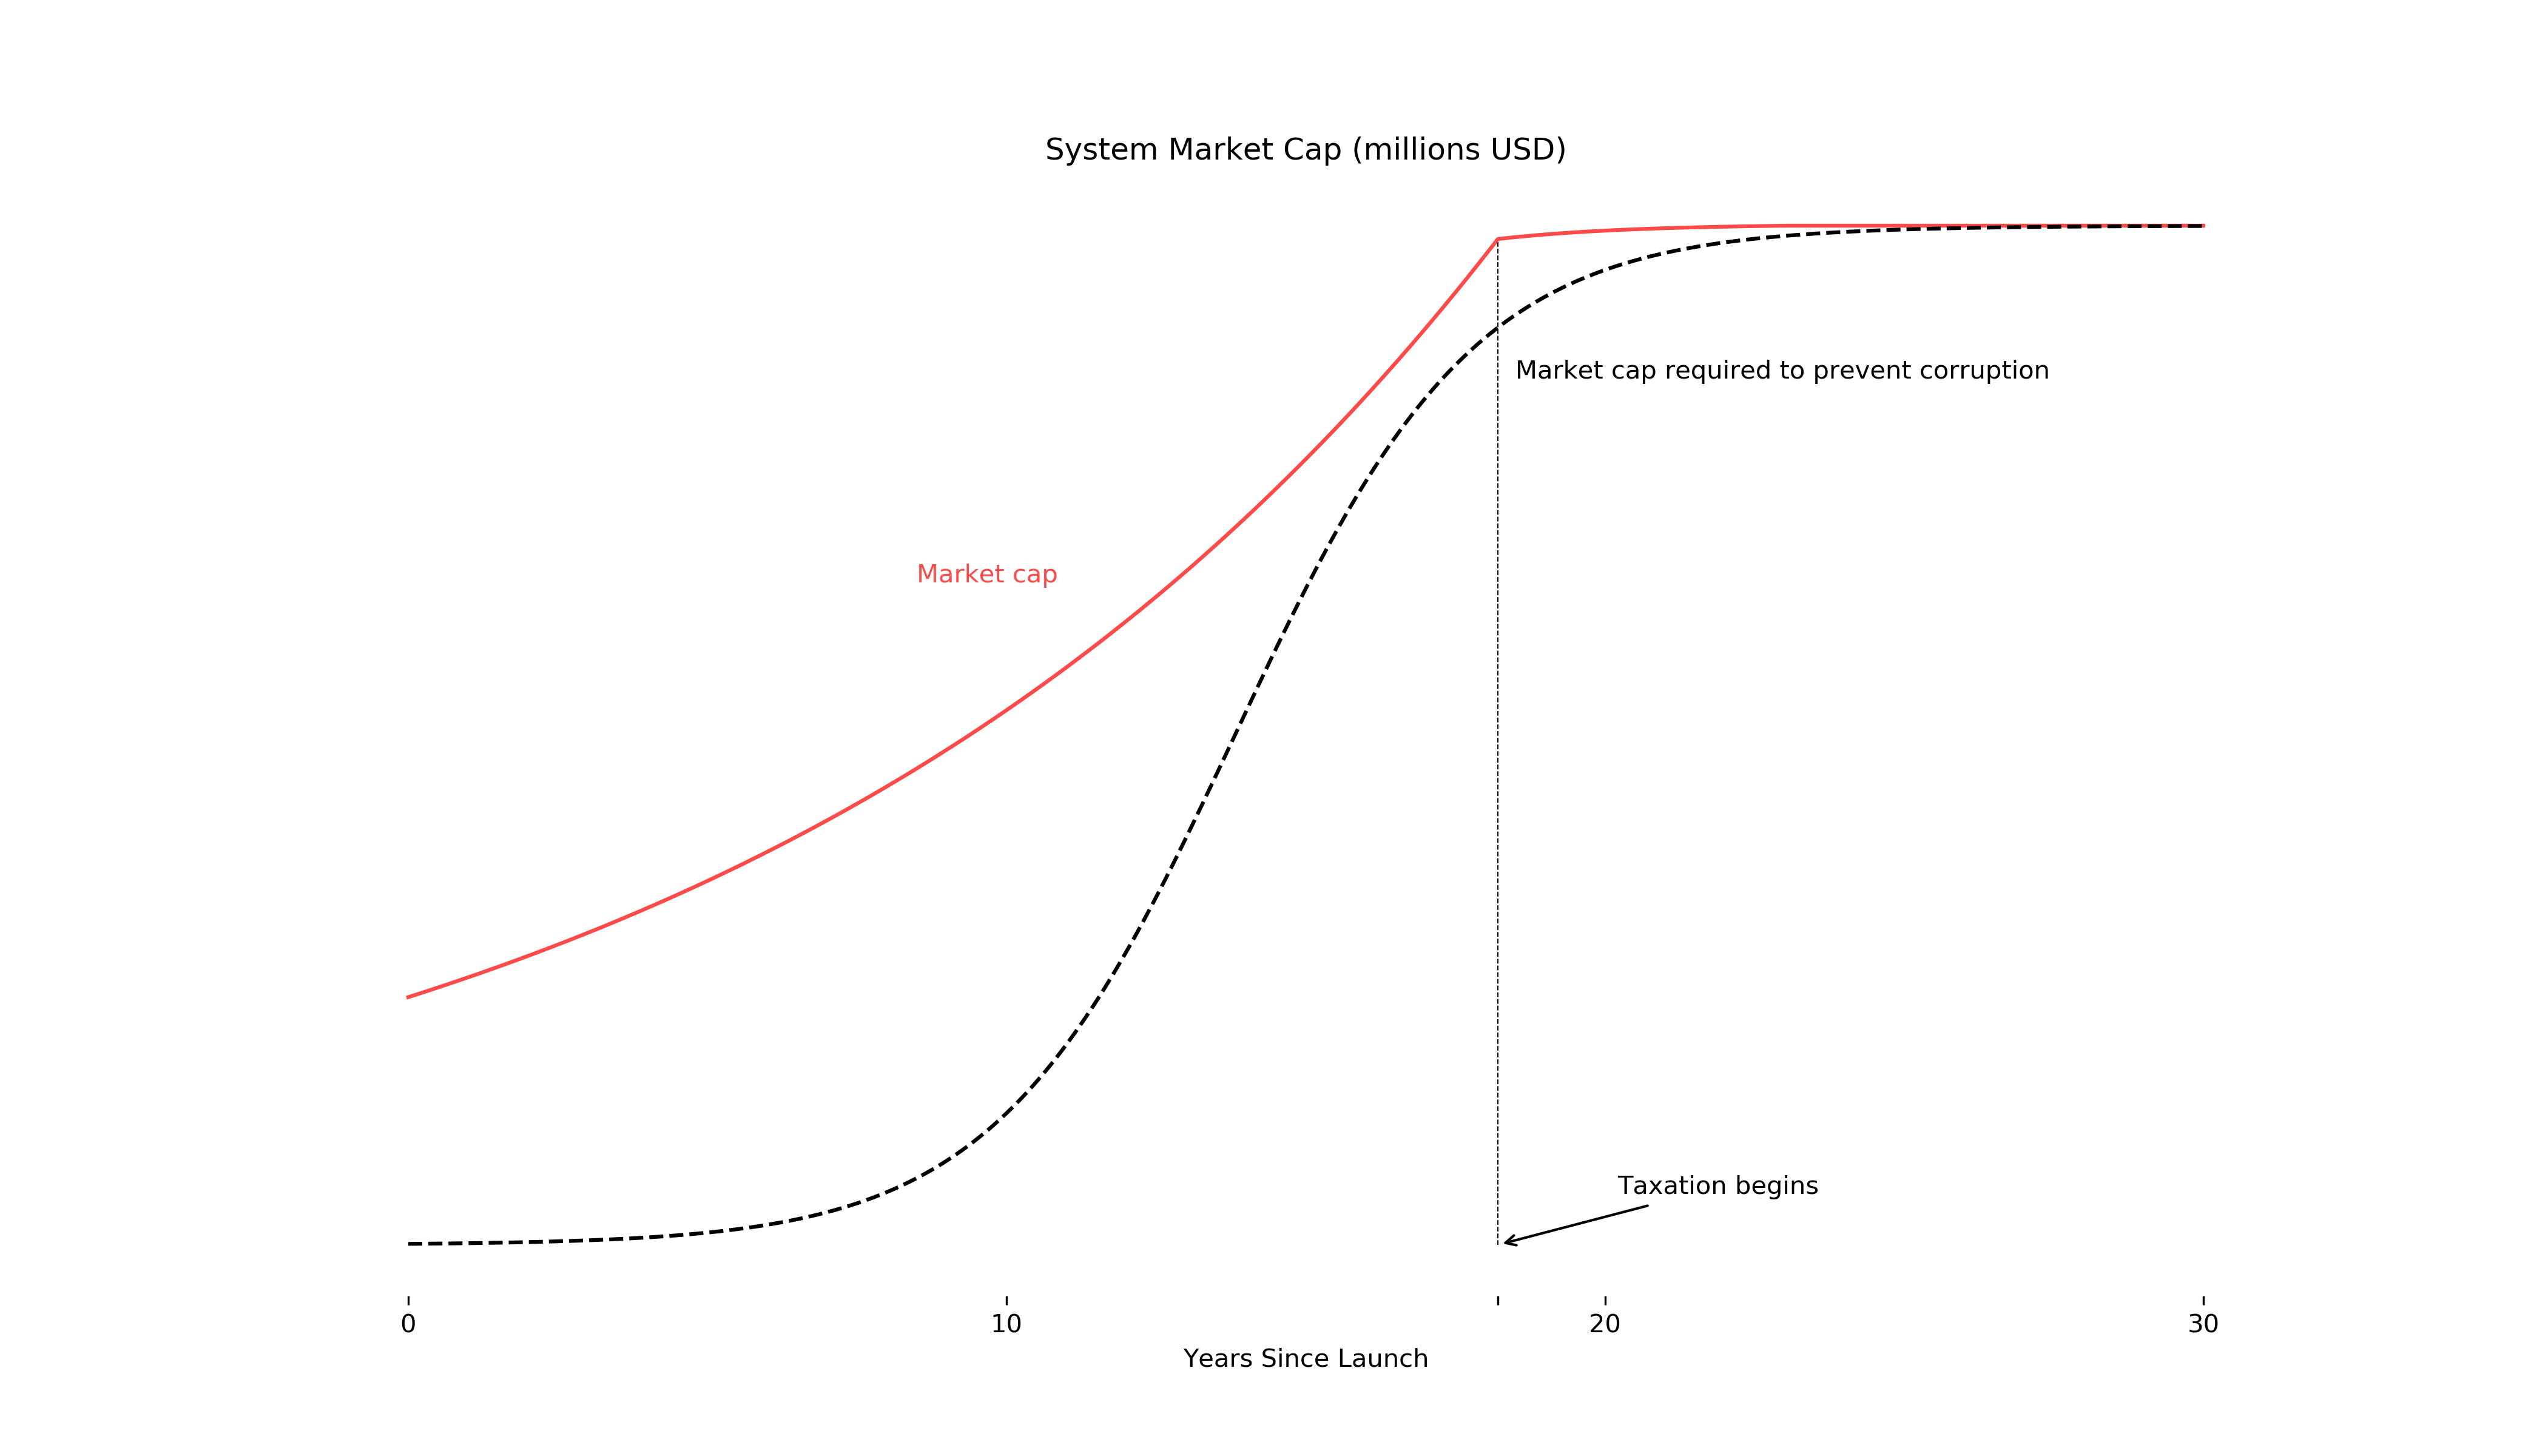
\includegraphics{../notes/TaxationPlanImages/MarketCap.png}}
      \label{fig:dg_tax_growth}
    \end{figure}

  \end{frame}


\section{Stochastic Model}

  \begin{frame} \frametitle{Stochastic Model}

    Up until now, everything has been completely deterministic

    \vspace{0.25cm}

    We now want to allow for margin growth to be stochastic

  \end{frame}

  \begin{frame} \frametitle{Margin process}

    We use a stochastic version of the logistic growth function

    \begin{figure}
      \scalebox{0.35}{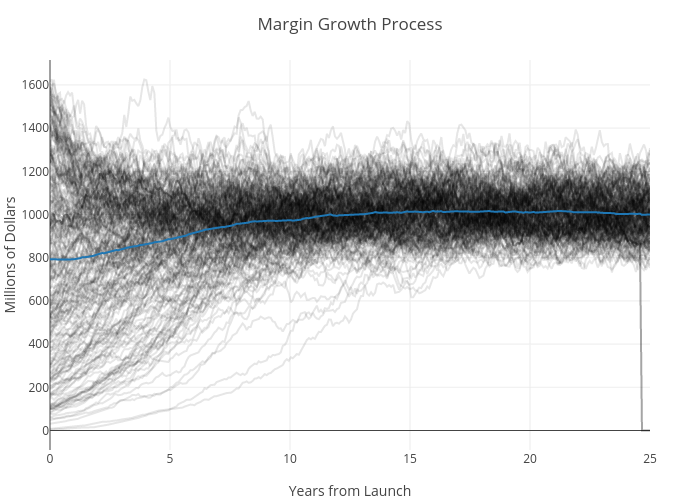
\includegraphics{../notes/TaxationPlanImages/StochasticMarginGrowth.png}}
    \end{figure}

  \end{frame}

  \begin{frame} \frametitle{Rainy day fund}

    Up until now, the buybacks and fees were equal $T_t = X_t$ which was an outcome of the
    fact that previous models were deterministic and margin was monotonically increasing

    \vspace{0.25cm}

    It will be important that we allow for them to not be equal going forward.

    \vspace{0.25cm}

    We introduce a new variable, $D_t$, as the ``rainy day fund'' that we have saved up prior to
    period $t$, then our period-by-period budget constraint is described by

    $$(1 + r) D_t + T_t \geq D_{t+1} + X_t$$

  \end{frame}

  \begin{frame} \frametitle{Choosing policy functions}

    We are allowed to pick two policies:

    \begin{enumerate}
      \item Buyback policy, $X^*(M_t)$
      \item Fee policy, $T^*(D_t, M_t)$
    \end{enumerate}

    \vspace{0.25cm}

    What are our goals in picking these?

    \vspace{0.25cm}

    We set out to find policies that minimize the present discounted value of buybacks performed and
    impose non-volatile, but low, fees.

  \end{frame}

  \begin{frame} \frametitle{Two step process}

    Hard to choose an objective function that accurately reflects both concerns at once, so we use
    a two step optimization process:

    \begin{enumerate}
      \item Find a buyback policy, $X^*(M_t)$, that minimizes the present discounted value of
            buybacks while still securing the system
      \item Find a fee policy, $T^*(D_t, M_t)$, that finds a low volatility tax policy which can
            fund the specified buyback policy
    \end{enumerate}

  \end{frame}

  \begin{frame} \frametitle{Formally...}

    \textbf{Step 1}:

    \begin{align*}
      \min_{X_t} \; & E \left[ \sum_{t} \left(\frac{1}{1 + r} \right) X_t \right] \\
      &\text{subject to} \\
      \quad & 2 PfC_t \leq E \left[ \sum_{s=0}^{\infty} \left(\frac{1}{1 + r}\right)^s X_{t+s} \right] \quad (\lambda_t) \\
      \quad & X_t \geq 0 \quad (\mu_t)
    \end{align*}

  \end{frame}

  \begin{frame} \frametitle{Formally...}

    \textbf{Step 2}:

    \begin{align*}
      \min_{\{T_t\}} \; & E \left[ \sum_{t} \left( \frac{1}{1 + r} \right)^t (T_t - \hat{\tau})^2 \right] \\
      &\text{subject to} \\
      T_t + (1 + r) D_t &\geq D_{t+1} + X^*_t \quad (\mu_t) \\
      D_t &\geq 0
    \end{align*}

  \end{frame}

  \begin{frame} \frametitle{Numerical Example: Baseline}

    We set the following parameters in our baseline case:

    \begin{itemize}
      \item One time period corresponds to one month
      \item Half of margin is seizable
      \item Annual risk-free interest rate of 2.5\%
      \item Target annualized fee of 2\% of margin
    \end{itemize}

  \end{frame}

  \begin{frame} \frametitle{Buyback policy and simulated buybacks}

    \begin{figure}
      \scalebox{0.35}{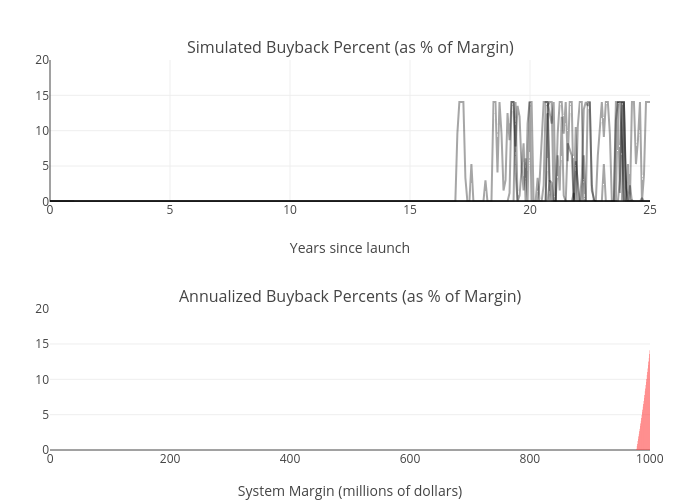
\includegraphics{../notes/TaxationPlanImages/StochasticBuybacks.png}}
    \end{figure}

  \end{frame}

  \begin{frame} \frametitle{Annualized Tax Rates}

    \begin{figure}
      \scalebox{0.35}{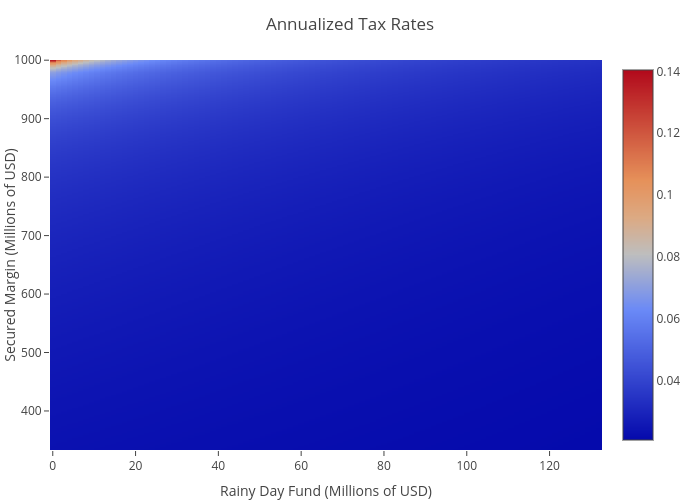
\includegraphics{../notes/TaxationPlanImages/AnnualizedTaxRates.png}}
    \end{figure}

  \end{frame}

  \begin{frame} \frametitle{Single simulation}

      \begin{figure}
        \scalebox{0.3}{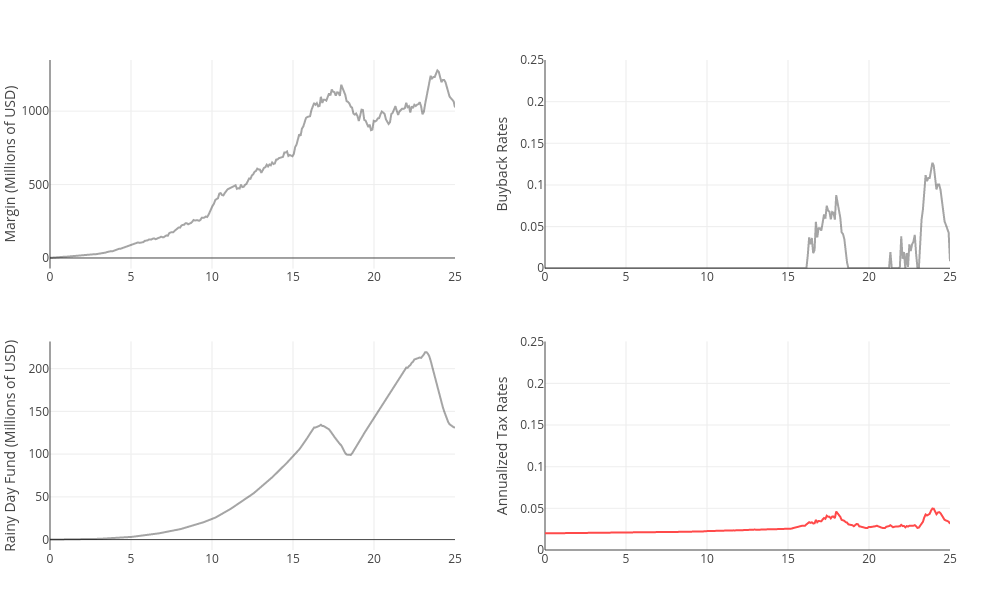
\includegraphics{../notes/TaxationPlanImages/SimulationPlots.png}}
        \label{fig:dg_tax_growth}
      \end{figure}

  \end{frame}


\section{Takeaways}

  \begin{frame} \frametitle{Two Takeaways}

    \begin{itemize}
      \item No reason to charge fees when system is small; the future expectation of buybacks can
            support system for a long time --- Even with added failure risk
      \item A rainy day fund plus optimal shape of buybacks allows for system to charge relatively
            low and non-volatile fees
    \end{itemize}

  \end{frame}

\end{document}
